\documentclass[]{article}

\usepackage{
	amsmath, 
	amssymb,
	float,
	graphicx,
	bera,
	parskip
}

\usepackage[
backend=biber, 
style=authoryear,
citestyle=apa, 
sorting=ynt]{biblatex}

\addbibresource{}
\graphicspath{ {Images/} }

\title{Assignment 7}
\author{
	Daniel Bok \\
	ESD \\
	1001049 \\
	daniel\_bok@mymail.sutd.edu.sg 
	\and
	Wong Yan Yee\\ 
	ISTD \\
	1001212 \\
	yanyee\_wong@mymail.sutd.edu.sg
	\and
	Clement Tan \\
	ESD \\
	1000948 \\
	clement\_tan@mymail.sutd.edu.sg
}
\date{\today}

\newcommand{\e}{&=}

\begin{document}
	
\maketitle
	
\section{Congestion and TCP}

\subsection{$U(x) = \log(x)$}
\begin{gather*}
\underset{x_a, x_1, x_2}{\max}\ \log(x_a) + \log(x_1) + \log(x_2) \\
s.t. \\
x_a + x_1 \leq C \\
x_a + x_2 \leq C \\
\end{gather*}
The reformulated problem with the Lagrangian can be written as
\begin{gather*}
L = \log(x_a) + \log(x_1) + \log(x_2) - \lambda_1(x_a + x_1 - C) - \lambda_2(x_a + x_2 - C) 
\end{gather*}
Taking derivatives of the Lagrangian:
\begin{gather*}
\begin{split}
\frac{dL}{dx_a} = 0 \\
\frac{1}{x_a} = \lambda_1 + \lambda_2
\end{split} \qquad 
\begin{split}
\frac{dL}{dx_1} = 0 \\
\frac{1}{x_1} = \lambda_1
\end{split} \qquad
\begin{split}
\frac{dL}{dx_2} = 0 \\
\frac{1}{x_2} = \lambda_2
\end{split} \\\\
\begin{split}
\frac{dL}{d\lambda_1} = 0 \\
x_a + x_1 = C
\end{split} \qquad
\begin{split}
\frac{dL}{d\lambda_2} = 0 \\
x_a + x_2 = C
\end{split}
\end{gather*}
Solving the systems of linear equations, we obtain
\begin{align*}
x_a + x_1 \e x_a + x_2 \\
x_1 \e x_2 \\
\frac{1}{x_a} \e \frac{1}{x_1} + \frac{1}{x_2} = \frac{2}{x_1} \\
x_a \e \frac{x_1}{2} = \frac{x_2}{2}
\end{align*}
Therefore, $x_a = \frac{C}{3}$ and $x_1 = x_2 = \frac{2C}{3}$.
	
\subsection{$U(x)=a\arctan(bx)$}

Given 
\[
	a = \frac{\sqrt{\frac{3}{2}}}{\sqrt{\frac{2}{3}}} = 1.5, b = 1, U(x) = 1.5 \arctan(x)
\]
The Lagrangian is given by:
\begin{gather*}
L = 1.5\arctan(x_a) + 1.5\arctan(x_1) + 1.5\arctan(x_2) - \lambda_1(x_a + x_1 - C) - \lambda_2(x_a + x_2 - C) \\
\end{gather*}
Taking derivatives of the Lagrangian:
\begin{gather*}
\begin{split}
\frac{dL}{dx_a} = 0 \\
\frac{1.5}{1 + x_a^2} = \lambda_1 + \lambda_2
\end{split} \qquad 
\begin{split}
\frac{dL}{dx_1} = 0 \\
\frac{1.5}{1 + x_1^2} = \lambda_1
\end{split} \qquad
\begin{split}
\frac{dL}{dx_2} = 0 \\
\frac{1.5}{1 + x_2^2} = \lambda_2
\end{split} \\\\
\begin{split}
\frac{dL}{d\lambda_1} = 0 \\
x_a + x_1 = C
\end{split} \qquad
\begin{split}
\frac{dL}{d\lambda_2} = 0 \\
x_a + x_2 = C
\end{split}
\end{gather*}
Solving the systems of linear equations, we obtain
\begin{align*}
x_a + x_1 \e x_a + x_2 \\
x_1 \e x_2 \\
\frac{1.5}{1 + x_a^2} \e \frac{1.5}{1 + x_1^2} + \frac{1.5}{1 + x_2^2} \\
\frac{1}{1 + x_a^2} \e \frac{2}{1 + x_1^2} \\
1 + x_a^2 \e \frac{1 + x_1^2}{2} \\
x_a \e \left| \sqrt{\frac{x_1^2 - 1}{2}} \right|
\end{align*}
To obtain the allocations, we will solve for
\begin{align*}
\sqrt{\frac{x_1^2 - 1}{2}} + x_1 \e C
\end{align*}

\subsection{$U(x) = x$}

We have the linear program given by:
\begin{gather*}
\underset{x_a, x_1, x_2}{\max}\ x_a + x_1 + x_2 \\
s.t. \\
x_a + x_1 \leq C \\
x_a + x_2 \leq C \\
\end{gather*}
The solution to the linear program is given by:
\begin{gather*}
x_a^* = 0 \qquad x_1^* = x_2^* = C
\end{gather*}

\subsection{Fair allocations}

Given that there are $n$ bottom users and assuming each link has the same capacity $C$,
\begin{description}
\item[$U(x) = \log(x)$] User A will receive $\frac{C}{n + 1}$ of the bandwidth . Users 1...n receive $\frac{Cn}{n+1}$ each.
\item[$U(x) = a \arctan (bx)$] User A will receive bandwidth proportional to $\sqrt{\frac{x_i^2 - 1}{n}}$. Users 1...n receive $C - \sqrt{\frac{x_i^2 - 1}{n}}$ each
\item[$U(x) = x$] User A will not get any bandwidth while all users 1... n will receive all the bandwidth they individually require.
\end{description}

Based on the consensus on fairness, we believe the allocations with $U(x) = \log(x)$ and $U(x) = a \arctan (bx)$ are still fair as they ensure every user gets a share of the network.


\section{A closer look at TCP}

By normal, we mean that the system is receiving the expected acknowledgement for each packet it sends.

\begin{figure}[H]
\centering
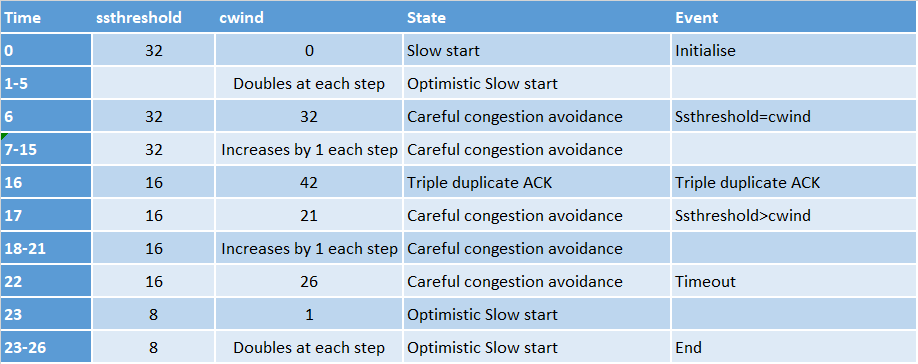
\includegraphics[width=\linewidth]{f1.png}
\end{figure}

\section{Long Fat Pipes}

\textbf{1. Why is it true that in general for TCP to use effectively a connection it must reach a window size at least equal to the BDP?}

The BDP represents the maximum amount of bits that can travel in the bottleneck link. This bottleneck link flow volume is also the constraint on the amount of bits that can travel in the whole connection. As such, for the connection to be utilized effectively, the window size should be at greater or equal to the BDP so that the maximum amount of packets can traverse the connection at any one time.

\textbf{2. In our specific case of single link network, is it true that the BDP is achieved when the sender transmits continuously at the maximum speed the link allows? Is it true that for physical reasons there is no way to increase further its window? Hence in this case BDP (in packets) is an upper bound on the maximum achievable window size?}

No. BDP may not be achieved even if the sender transmit at the maximum speed the link allows. The sender is also limited by his window size ($2^{16}$ bytes) which could be much smaller than the BDP. In that case, the sender does not reach BDP and is not using the connection effectively.

No. Since the BDP of the link can be much greater than the TCP-allowed window size, it is not for physical reasons that there is no way to increase the window size. Rather, it is the constraint on the TCP header itself.

In this case, BDP is not an upper bound on the maximum achievable window size, rather it is the TCP header. However, if the BDP were to fall below the size specified by the TCP header, it would be the upper bound.

\textbf{3. Assuming your answer is yes in the previous question, and that a single TCP connection is using the link, is it true that the evolution of its window size W is extremely simple: increase linearly from zero until $W	= min(MAX, BDP)$ and then stay constant at this maximum value?}

No. We assume first that the BDP is smaller than $2^{16}$. Since the connection has no idea what the BDP of the link is, it will always try to increase the window size when it can. When the moment the window is increased to BDP + 1, the connection will sense congestion and immediately half the window size. This AIMD pattern implies that there is no time when the packet transmission rate is constant.

If the BDP is greater than the $2^{16}$ (window size), then the connection will hit a constant output rate as its window size is fixed to a maximum specified in the TCP header.

\textbf{4. Consider a local LAN link such as an Ethernet link, connecting the sender and the receiver with 10Mbps, and $RTT_d$ = 2ms. What is the BDP? Is TCP eventually constrained by MAX or BDP? What is the maximum rate achievable? How much time does it take to reach this maximum rate?}

\begin{align*}
BDP \e BW \cdot RTT_d = 10^7 \cdot 2 \cdot 10^{-3} \\
	\e 2 \cdot 10^4\ \text{bytes} \\
	\e \frac{2 \cdot 10^4}{1460} \approx 14\ \text{packets}
\end{align*}

Since the maximum number of packets sent (14) is less than that allowable by the TCP header, the connection is constrained by BDP. The maximum achievable rate is around 14 packets per window. 

It takes approximately $14 \cdot 2ms = 28ms$ to reach this maximum rate.

\textbf{5. Consider a fibre optic link of 10 Gbps and $RTT_d$ = 20ms. Repeat the previous questions.	What do you observe?}

\begin{align*}
BDP \e 10^{10} \cdot 20\cdot 10^{-3} \\
	\e 2 \cdot 10^8\ \text{bytes}\\
	\e \frac{2 \cdot 10^8}{1460} \approx 137000\ \text{packets}
\end{align*}

We notice that by increasing the bandwidth and the latency ($RTT_d$), we can can make the TCP window size (=$2^{16}$) the limiting factor. 

\textbf{6. Suppose we remove the constraint that TCP uses the MAX window size, i.e., we set MAX = $\infty$. Repeat the previous question. What is the main issue here?}

Since the MAX = $\infty$, BDP becomes the limiting factor. The issue with this is that the linear growth rate is too slow to effectively maximize the connection. Given a latency of 20ms, it would take approximately $137000 \cdot 20ms \approx 46\ \text{minutes}$ to achieve the maximum throughput rate. 

\textbf{7. Suppose that we double the window size every $RTT_d$	(again assuming MAX = $\infty$). How much time does it take to reach the maximum rate?}

\begin{align*}
T \e 20 \cdot 10^{-3} \cdot \log_2 137000 \\
	&\approx 0.34\ \text{seconds}
\end{align*}

\textbf{Think of the time it takes to transmit a file of say 20 Mbytes. Compare the time it takes if we use TCP (as in the previous question) and the time if we could use 100\% of the 10Gbps link}

Given each packet is 1460 bytes, the file will have a total of 
\[
\frac{20 \cdot 10^6 }{1460} \approx 13700\ \text{packets} 
\]

If we were to use TCP with $MAX = \infty$, the time taken is given by
\begin{gather*}
\min T \\
st. \sum_{i=1}^{T} 2^{i-1} \geq 13700 \\
T^* = 14 \cdot 20ms = 280ms
\end{gather*}

If we used 100\% of the 10Gbps link straight away, we only need 20ms. This is because we are sending all our packets through the link in one instance.

\end{document}
